\documentclass[11pt,twoside,notitlepage]{book}

\RequirePackage{lineno}
\usepackage{import}
\usepackage{titlesec}
\usepackage{enumitem}
\usepackage{amssymb, amsmath}
\usepackage{mathpazo}
\usepackage{float,graphicx}
\graphicspath{{./figs}}
\usepackage[figuresright]{rotating}
\usepackage[usenames,dvipsnames]{color}
\usepackage{microtype}
\usepackage{tabulary}
\usepackage{booktabs,multirow,dcolumn,bigdelim}
\newcommand{\otoprule}{\midrule[\heavyrulewidth]}
\usepackage{xr-hyper}
\usepackage[pdftex,plainpages=false,pdfpagelabels,backref,pdfborder={0 0 0}]{hyperref}
%\externaldocument{ReviewResponses/DOE_review_responses_11202014}
\usepackage{url}
\usepackage[toc,page,titletoc]{appendix}
\usepackage{afterpage}
\usepackage[font=small,labelfont=bf]{caption}
\setlength\captionmargin{15pt}
\usepackage[scaled]{helvet}
\usepackage{sectsty}
\allsectionsfont{\normalfont\sffamily}
\usepackage{titletoc}
\titlecontents{chapter}
  [1.5em]
  {\linespread{0.9}\normalfont\sffamily\bfseries}
  {\contentslabel{1em}} 
  {\hspace*{-2.3em}} 
  {\mdseries\titlerule*[1pc]{.}\contentspage} 
\titlecontents{section}
  [3.5em]
  {\linespread{0.9}\normalfont\sffamily}
  {\contentslabel{2.3em}} 
  {\hspace*{-2.3em}} 
  {\titlerule*[1pc]{.}\contentspage} 
\titlecontents{subsection}
  [4.5em]
  {\linespread{0.9}\normalfont\sffamily}
  {\contentslabel{2.3em}} 
  {\hspace*{-2.3em}} 
  {\titlerule*[1pc]{.}\contentspage} 
\titlecontents{subsubsection}
  [5.5em]
  {\linespread{0.9}\normalfont\sffamily}
  {\contentslabel{2.3em}} 
  {\hspace*{-2.3em}} 
  {\titlerule*[1pc]{.}\contentspage} 
\tolerance = 10000

\usepackage[text={6.5in,8.75in},headheight=15pt,centering]{geometry}
\usepackage{xspace}

\DeclareGraphicsExtensions{.pdf,.png}
\newcommand{\filenamedot}{.}
\setlength{\parindent}{0.0in}
\setlength{\parskip}{0.1in}
\renewcommand{\topfraction} {0.9}
\renewcommand{\bottomfraction} {0.9}
\renewcommand{\textfraction} {0.1}
\renewcommand{\floatpagefraction} {0.8}

\usepackage{fancyhdr}
\pagestyle{fancy}
\renewcommand{\chaptermark}[1]{\markboth{#1}{}}
\renewcommand{\sectionmark}[1]{\markright{#1}{}}
\fancyhead{} % clear all header fields 
\fancyhead[RO,LE]{\sffamily \rightmark}
\fancyhead[LO,RE]{\sffamily \leftmark}
\fancyfoot{} % clear all footer fields 
\fancyfoot[RO,LE]{\sffamily \thepage}
\renewcommand{\headrulewidth}{0pt} 
\fancypagestyle{plain}{%
  \fancyhf{}
  \fancyfoot[RO,LE]{\sffamily \thepage}
}

\usepackage{eurosym}
\usepackage{xcolor}
\usepackage{framed}
\colorlet{shadecolor}{blue!10}

\setcounter{secnumdepth}{2}
\setcounter{tocdepth}{1}

\newcommand{\lyxdot}{.}
\usepackage{subfig}

\setlength\fboxsep{0pt}
\setlength\fboxrule{0.5pt}
\title{sPHENIX baseline scope}
\begin{document} 

%\linenumbers

\frontmatter

\pagestyle{empty}
\renewcommand*\familydefault{\sfdefault}
{\sffamily
\vfill
\vspace{4cm}
\begin{figure}[H]
  \begin{center}
    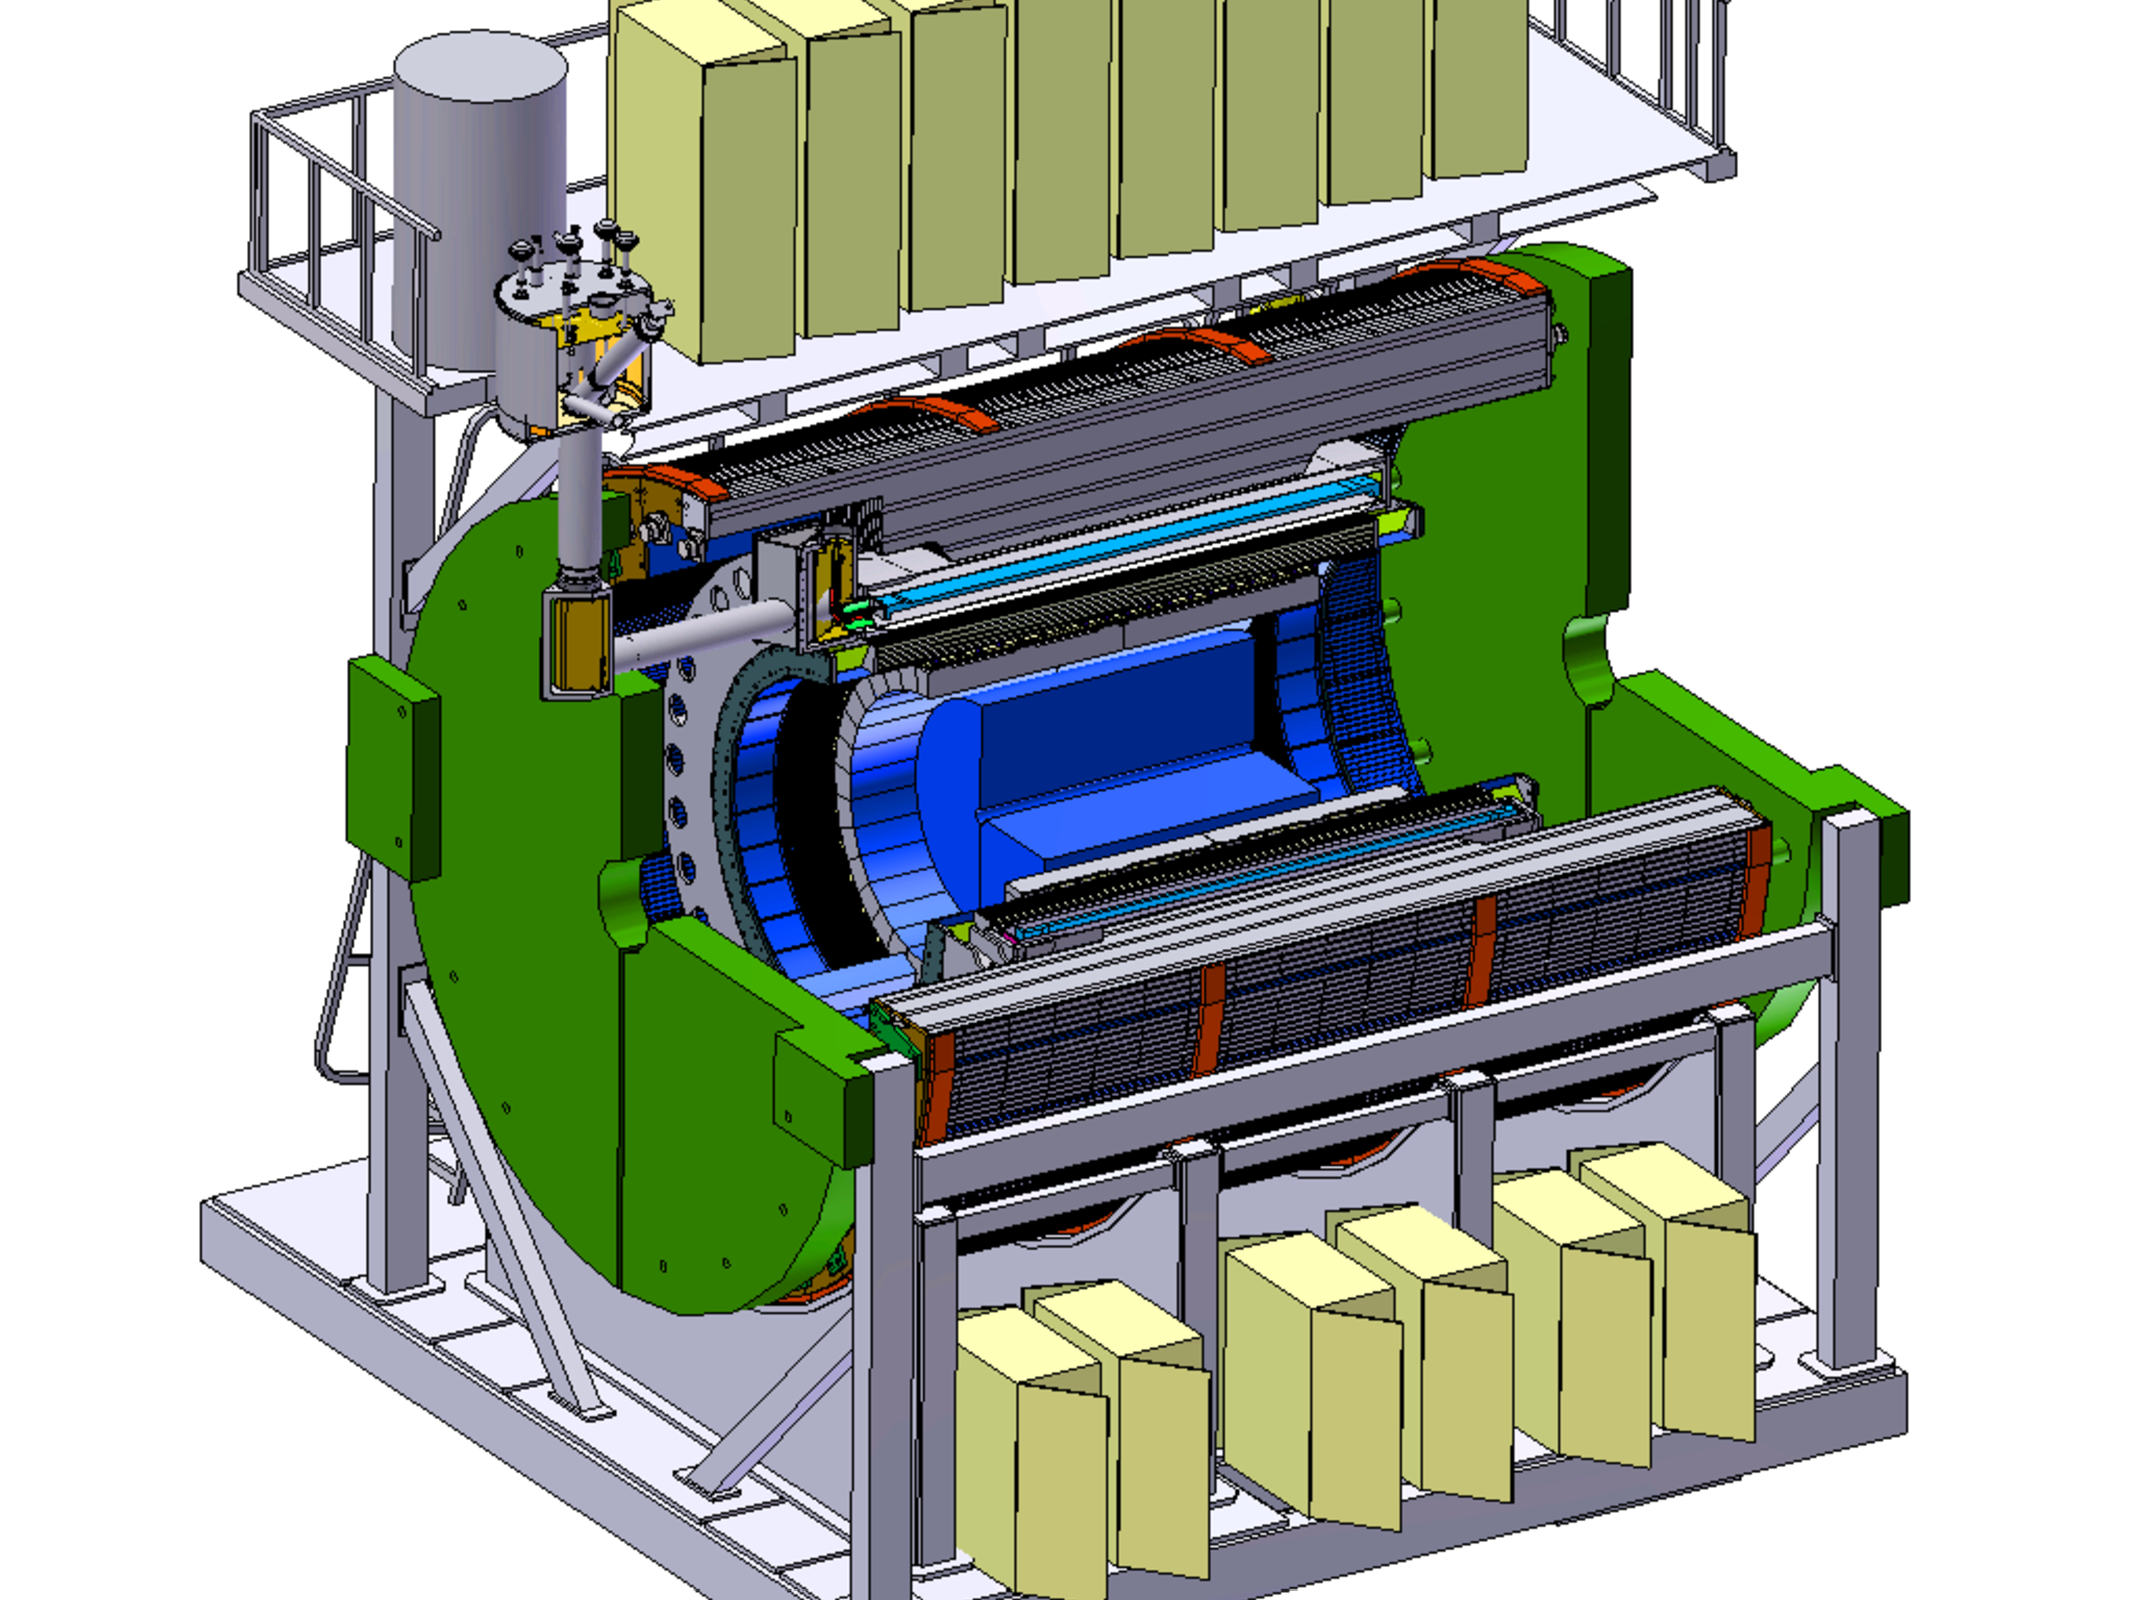
\includegraphics[width=\linewidth]{figs/sPHENIX}
  \end{center}
\end{figure}

\begin{center}
  \LARGE
  \vskip 2 em
  Addressing the Baseline Scope Charge\\
  \vskip 4 em
  The sPHENIX Collaboration \\
  May 31, 2016 \\
\end{center}

\vspace{2cm}

\begin{figure}[H]
  \begin{center}
    %\includegraphics[width=0.7\linewidth]{figs/cover}
  \end{center}
\end{figure}
}


\vfill
\renewcommand*\familydefault{\rmdefault}


\cleardoublepage
\pagestyle{fancy}
\section*{Executive Summary}
\label{executive_summary}
\setcounter{page}{1}

\nocite{*}

In this document the sPHENIX collaboration answers a charge~(see
Appendix~\ref{charge}) from BNL ALD Berndt Mueller to develop
a baseline design scope that provides a compelling phsyics program
within the constraints of possible DOE funding redirected from 
RHIC operations. The document describes a reference design aimed
at a compelling program focussed on three science drivers: jet structure,
heavy-flavor jet production and $\Upsilon$ spectroscopy. We then
provide a comprehensive list of re-scoping options for each
of the main subdetector systems, and describe the associated
cost savings, the engineering and schedule impact and impact on 
key performane measures related to the three science 
drivers. Based on these criteria, we develop examples of 
rank-ordered lists of re-scoping options including the 
cumulative cost-savings and science impact.




\cleardoublepage

\resetlinenumber

\tableofcontents
\cleardoublepage

\mainmatter

\renewcommand{\thepage}{\arabic{page}}
\setcounter{chapter}{0}
\setcounter{page}{1}

\cleardoublepage

\appendix

\chapter*{Charge}
\label{charge}

\begin{figure}[hbt!]
  \centering
  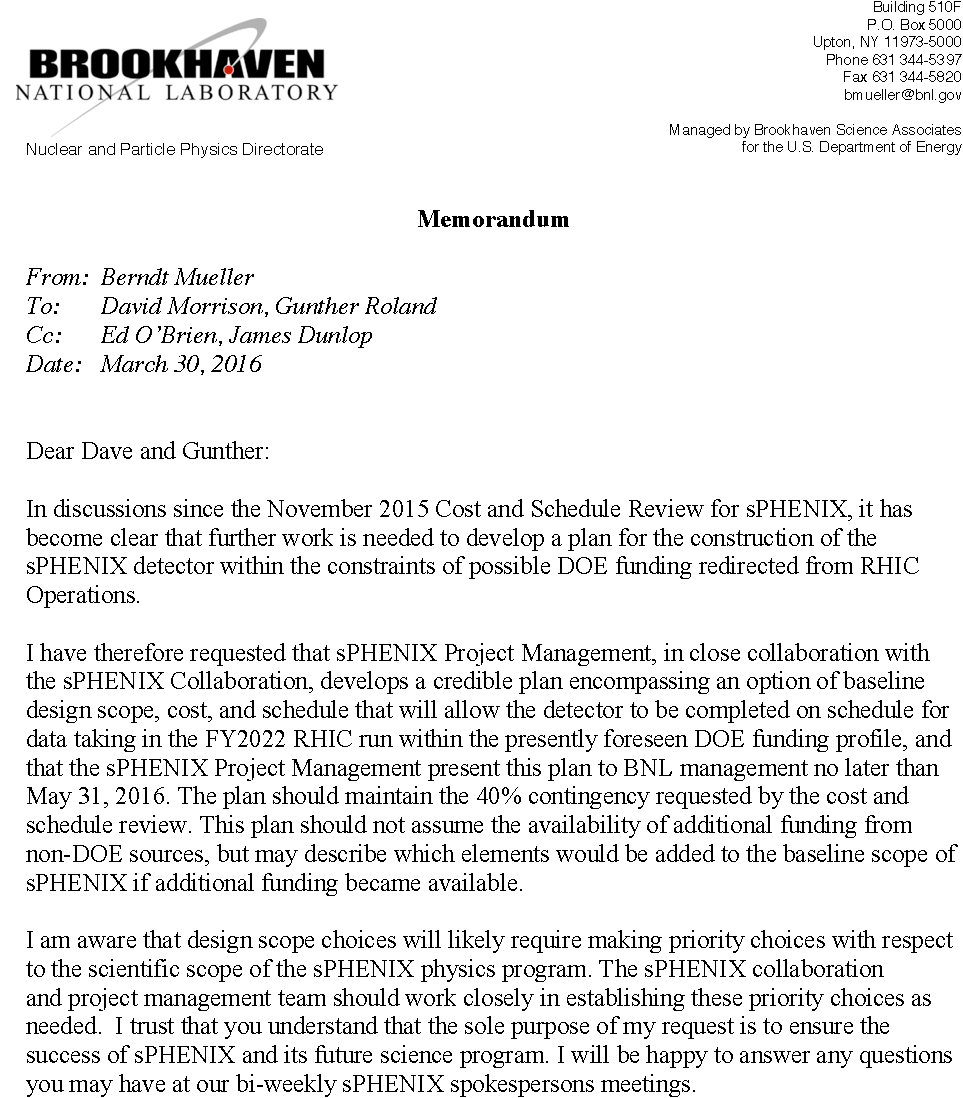
\includegraphics[width=0.8\linewidth]{charge_memo}
\end{figure}



\cleardoublepage

\backmatter

\cleardoublepage
\phantomsection
\addcontentsline{toc}{chapter}{List of Tables}
\listoftables

\cleardoublepage
\phantomsection
\addcontentsline{toc}{chapter}{List of Figures}
\listoffigures

\cleardoublepage
\phantomsection
\addcontentsline{toc}{chapter}{References}

\bibliographystyle{unsrturl}
\bibliography{refs}

\end{document} 


